% -*- latex -*-
%%%%%%%%%%%%%%%%%%%%%%%%%%%%%%%%%%%%%%%%%%%%%%%%%%%%%%%%%%%%%%%%
%%%%%%%%%%%%%%%%%%%%%%%%%%%%%%%%%%%%%%%%%%%%%%%%%%%%%%%%%%%%%%%%
%%%%
%%%% This text file is part of the lecture slides for
%%%% `Parallel Programming in MPI and OpenMP'
%%%% by Victor Eijkhout, copyright 2012-6
%%%%
%%%% Tasks-slides.tex : slides about OpenMP workshare constructs
%%%%
%%%%%%%%%%%%%%%%%%%%%%%%%%%%%%%%%%%%%%%%%%%%%%%%%%%%%%%%%%%%%%%%
%%%%%%%%%%%%%%%%%%%%%%%%%%%%%%%%%%%%%%%%%%%%%%%%%%%%%%%%%%%%%%%%

\begin{frame}[containsverbatim]{More flexibility}
  \begin{itemize}
  \item You have seen loops and sections.
  \item How about linked lists or trees?
  \item Tasks are very flexible:\\
    you create work, it goes on a queue, gets executed later
  \end{itemize}
\begin{verbatim}
p = head_of_list();
while (!end_of_list(p)) {
#pragma omp task
  process( p );
  p = next_element(p);
}
\end{verbatim}
\end{frame}

\begin{frame}{Threads, tasks, queues}
  \begin{itemize}
  \item There is one queue (per team), not visible to the programmer.
  \item One thread starts generating tasks.
  \item Tasks can recursively generate tasks.
  \item You never know who executes what.
  \end{itemize}
  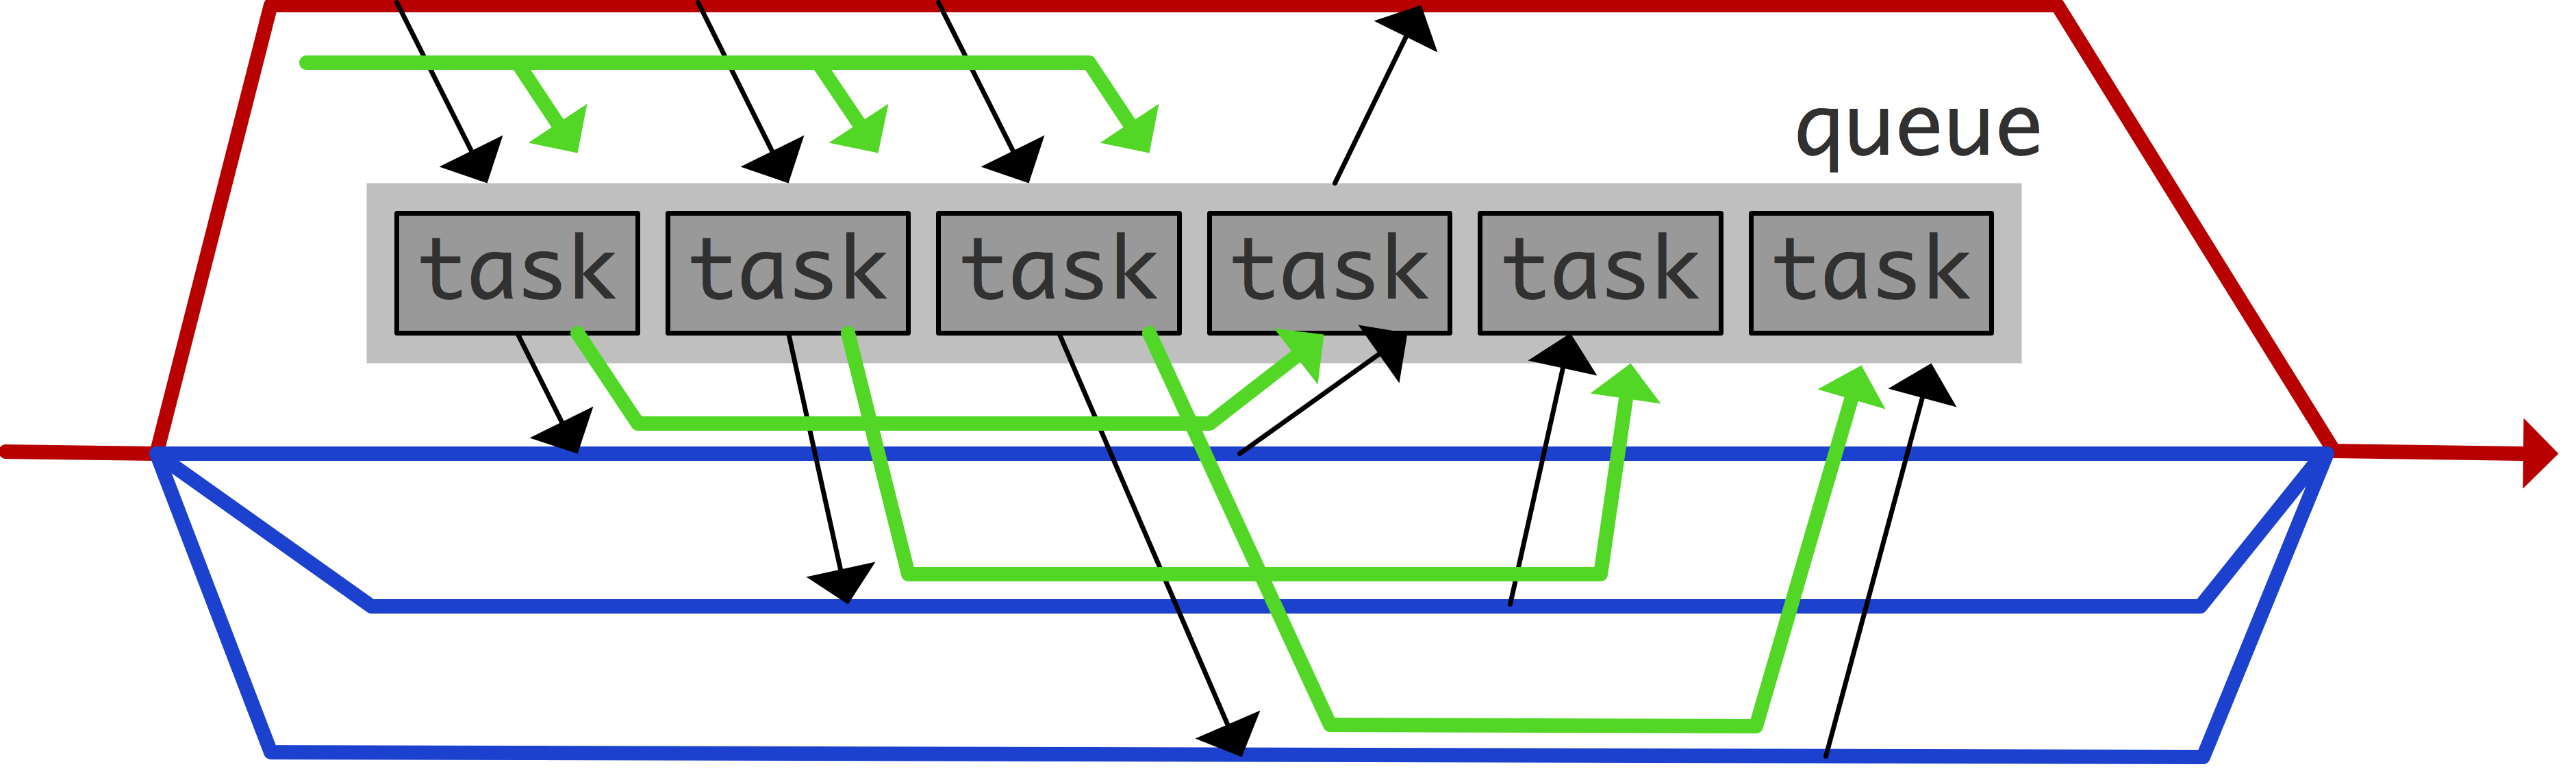
\includegraphics[scale=.1]{taskthread}
\end{frame}

\begin{exerciseframe}[taskfactor]
  \input ex:taskfactor
\end{exerciseframe}

\begin{frame}[containsverbatim]{Task synchronization}
  Mechanisms for task synchronization:
  \begin{itemize}
  \item \indextermtt{taskwait}: wait for all previous tasks (not nested)
  \item \indextermtt{taskgroup}: wait for all tasks, including nested
  \item \indextermtt{depend}: synchronize on data items.
  \end{itemize}
\end{frame}

\begin{frame}[containsverbatim]{Example: tree traversal}
\begin{verbatim}
int process( node n ) {
  if (n.is_leaf)
    return n.value;
  for ( c : n.children) {
#pragma omp task
    process(c);
#pragma omp taskwait
  return sum_of_children();
}
\end{verbatim}
\end{frame}

\begin{frame}[containsverbatim]{Example: Fibonacci}
\begin{verbatim}
long fib(int n) {
  if (n<2) return n;
  else { long f1,f2;
#pragma omp task
  f1 = fib(n-1);
#pragma omp task
  f2 = fib(n-2);
#pragma omp taskwait
  return f1+f2;
}

#pragma omp parallel
#pragma omp single
  printf("Fib(50)=%ld",fib(50));
\end{verbatim}
(what is conceptually wrong with this example?)
\end{frame}

\begin{frame}[containsverbatim]{Fibonacci once more}
\begin{verbatim}
long fibs[100];
void fib(n) {
  if (n>=2) {
    #pragma omp task \
       depend( in:fibs[n-2],in:fibs[n-1] ) \
       depend( out:fibs[n] )
    fibs[n] = fibs[n-2]+fibs[n-1];
};

#pragma omp parallel
#pragma omp single
  for (i<50)
    fib(i);
\end{verbatim}
\end{frame}

\endinput

\begin{frame}[containsverbatim]{}
  \begin{itemize}
  \item 
  \end{itemize}
\end{frame}

\endinput

\begin{frame}[containsverbatim]{}
  \begin{itemize}
  \item 
  \end{itemize}
\end{frame}

